\documentclass{article}
\usepackage{graphicx} % Required for inserting images
\usepackage{grffile} % Allow spaces in image file names
\usepackage{float}
\setcounter{secnumdepth}{0}
\usepackage{listings}

\title{Sequential RISC-V Processor Design}
\author{
\begin{tabular}{ccc}
Sanjana Punna & Saikiran S & Himangi Sahoo \\
2024102065 & 2024112007 & 2024112020
\end{tabular}
}
\date{February 2026}
\usepackage[hidelinks]{hyperref}
\begin{document}

\maketitle
\tableofcontents
\newpage

\section{Introduction}
A sequential processor (also known as a non-pipelined processor) executes every instruction step-by-step in a single processing unit. In this design, the entire instruction completes before the next one begins. Hence, at any moment in time, only one instruction is active inside the CPU.

Our processor only supports the following instructions:
\textbf{add}, \textbf{sub}, \textbf{addi}, \textbf{and}, \textbf{or}, \textbf{ld}, \textbf{sd} and \textbf{beq}.
\begin{figure}[H]
    \centering
    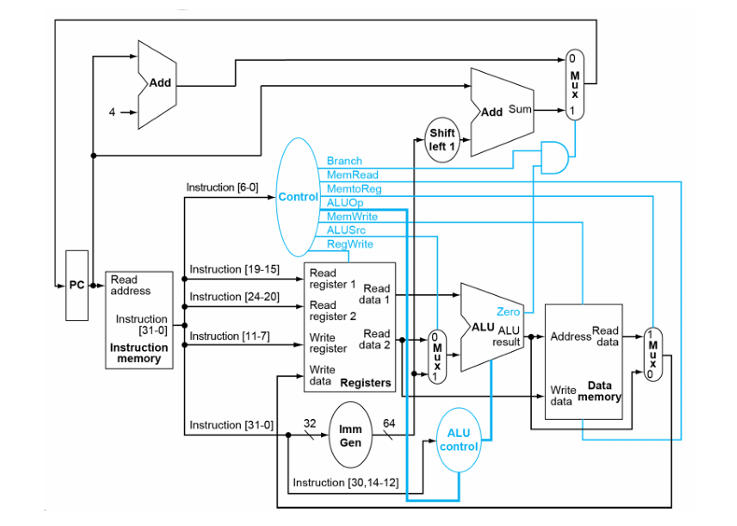
\includegraphics[width=1.1\linewidth]{Processor Outline.png}
    \caption{Sequential Datapath}
    \label{fig:placeholder}
\end{figure}
\noindent Although the processor is sequential, each instruction still goes through the following five logical stages. The five stages are:
\begin{enumerate}
    \item {Instruction Fetch(IF)}
    \item {Instruction Decode(ID)}
    \item {Execute(EX)}
    \item {Memory Access (MEM)}
    \item {Write Back (WB)}
\end{enumerate}
    
\section{Stage 1: Instruction Fetch}
This stage is responsible for retrieving the next instruction from the memory.
\begin{figure}[H]
    \centering
\fbox{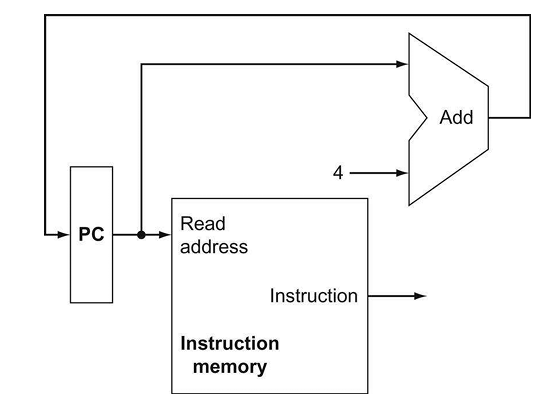
\includegraphics[width=0.6\linewidth]{Stage1.png}}
    \caption{PC and Instruction memory}
    \label{fig:placeholder}
\end{figure}
        
        \subsection{Program Counter(PC):-}
        \begin{itemize}
            \item The Program Counter (PC) is a 64-bit register which holds the address of the instruction to be executed.
                \item It is basically a pointer which points to the address of the next executable instruction.
                \item The PC is updated by 4 after each 32-bit (4 bytes) instruction  to point to the next instruction. This is done by using an adder.
            \item The PC is incremented to point to the next instruction.
            \item A multiplexer (MUX) selects between the next sequential instruction address (PC + 4) and the branch target address, depending on the branch control signal.
            \end{itemize}
        \subsubsection*{\textbf{Verification:}}
            The module has been implemented in verilog and has been verified with an appropriate test bench. The output verifying the test-cases is as follows:-
            \begin{figure}[H]
            \centering
            {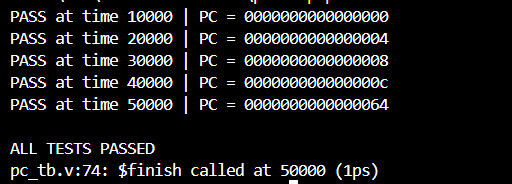
\includegraphics[width=0.6\linewidth]{PC_Verify.png}}
                \caption{Sample Testbench output of Program Counter (PC)}
                \label{fig:placeholder}
            \end{figure}
            
            \subsection{Instruction memory(IR):-}
            \begin{itemize}
                \item The address of the next instruction is passed to the Instruction memory.
                \item It fetches the instructions from the memory and sends the 32-bit instruction to the next stage .i.e, the Instruction Decode Stage.
            \end{itemize}
            \subsubsection*{\textbf{Verification:}}
            The module has been implemented in verilog and has been verified with an appropriate test bench. The output verifying the test-cases is as follows:-
            \begin{figure}[H]
                \centering
                {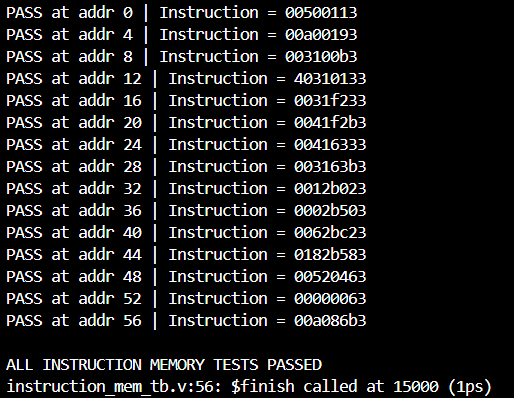
\includegraphics[width=0.6\linewidth]{INSTRUCTION_TEST.png}}
                    \caption{Sample Testbench output of Instruction Memory}
                    \label{fig:placeholder}
            \end{figure}  
        
\section{Stage 2: Instruction Decode}
This stage decodes the fetched instruction to make the processor identify the required operands for execution, by extracting the opcode, register addresses, immediate values etc.
\begin{figure}[H]
    \centering
\fbox{    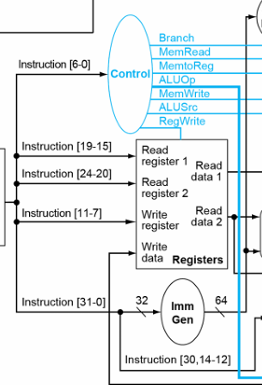
\includegraphics[width=0.4\linewidth]{Stage 2.png}}
    \caption{Instruction Decode}
    \label{fig:placeholder}
\end{figure}
            \subsection{Control Unit:-}
            \begin{itemize}
                \item The control unit decodes the instruction to determine its meaning - it receives the Opcode [6:0] and generates the corresponding control signals.
                \item The Opcodes are as follows :-
                \begin{table}[h]
                    \centering
                    \begin{tabular}{c|c}
                         Instruction & Opcode \\ \hline
                         R-type & 0110011 \\
                         Load & 0000011 \\
                         Store & 0100011 \\
                         Branch & 1100011 \\
                         \hline
                    \end{tabular}
                    \label{tab:placeholder}
                \end{table}
                \item Identifies the required registers and addressing modes.
                \item Selects the ALU operation or control signals needed for execution.
            \end{itemize}
            \subsubsection*{\textbf{Verification:-}}
            The module has been implemented in verilog and has been verified with an appropriate test bench. The output verifying the test-cases is as follows:-
             \begin{figure}[H]
                    \centering
                    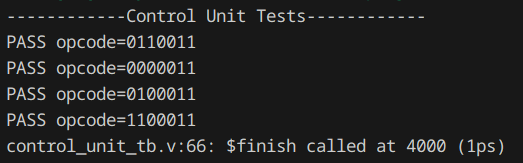
\includegraphics[width=0.6\linewidth]{ctrl.png}
                    \caption{Sample Testbench output of Control Unit}
                    \label{fig:placeholder}
                \end{figure}
            
            \subsection{Registers:-}
            \begin{itemize}
                \item Bits [19:15] and [24:20] are used to read values from the Register File.
                \item Bits [11:7] are used to store result in the Register File after the operation is executed.
            \end{itemize}
            \subsubsection*{\textbf{Verification:-}}
            The module has been implemented in verilog and has been verified with an appropriate test bench. The output verifying the test-cases is as follows:-
             \begin{figure}[H]
                    \centering
                    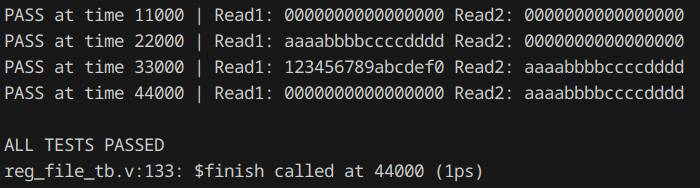
\includegraphics[width=0.6\linewidth]{reg.png}
                    \caption{Sample Testbench output of Register}
                    \label{fig:placeholder}
                \end{figure}
            \subsection{Immediate Generator:-}
            \begin{itemize}
                \item It extracts the immediate values for load, store, I-type and B-type instructions.
                \item it converts the immediate values from 32-bit to 64-bit - it just extends the last bit till 64-bits.
                \begin{figure}[H]
                    \centering
                    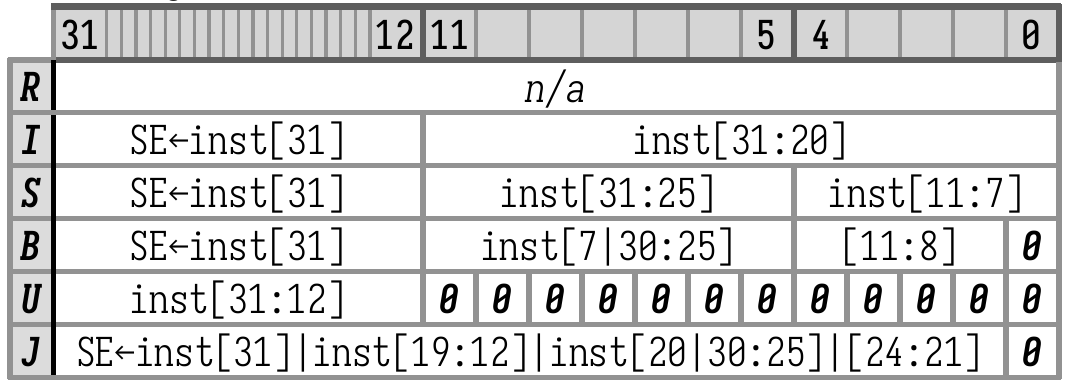
\includegraphics[width=0.7\linewidth]{Screenshot_20260222_165548.png}
                    \caption{32-bit Immediate value bits for different types of instruction}
                    \label{fig:placeholder}
                \end{figure}
            \end{itemize}
            \subsubsection*{\textbf{Verification:-}}
            The module has been implemented in verilog and has been verified with an appropriate test bench. The output verifying the test-cases is as follows:-
             \begin{figure}[H]
                    \centering
                    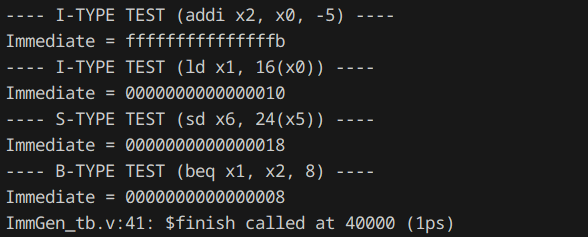
\includegraphics[width=0.6\linewidth]{immgen.png}
                    \caption{Sample Testbench output of Immediate Generator}
                    \label{fig:placeholder}
                \end{figure}
\section{Stage 3: Execution}
This stage fetches the data from the registers and executes the operation decoded by the Instruction Decode Stage.
\begin{figure}[H]
    \centering
   \fbox{ 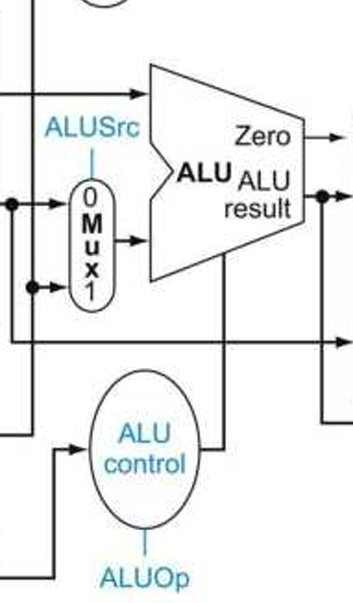
\includegraphics[width=0.3\linewidth]{Stage 3.png}}
    \caption{ALU Control and ALU}
    \label{fig:placeholder}
\end{figure}
            \subsection{ALU Control Unit:-}
            \begin{itemize}
                \item It fetches the ALUOp code from Control Unit to determine the type of instruction to be operated i.e. S-type, I-type, B-type etc.
                \item Based on instruction code [31:0], it determines which operation to perform i.e Add, Subtract, AND, OR, by decoding the funct7 and funct3 field.
                \item Generates a 4-bit instruction which corresponds to which operation to execute.
                \item The 4-bit instructions with its corresponding function is as follows :-
                \begin{table}[h]
                    \centering
                    \begin{tabular}{c|c}
                         ALU control lines & Function \\ \hline
                         0000 & AND \\
                         0001 & OR \\
                         0010 & Add \\
                         0110 & Subtract \\
                         \hline
                    \end{tabular}
                    \label{tab:placeholder}
                \end{table}
                \begin{figure}[H]
                    \centering
                    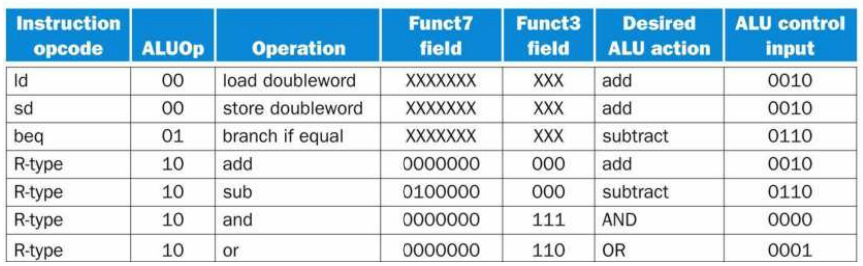
\includegraphics[width=0.8\linewidth]{2.png}
                    \caption{ALUOp, ALU control lines and its corresponding functions}
                    \label{fig:placeholder}
                \end{figure}
            \end{itemize}
            \subsubsection*{\textbf{Verification:-}}
            The module has been implemented in verilog and has been verified with an appropriate test bench. The output verifying the test-cases is as follows:-
             \begin{figure}[H]
                    \centering
                    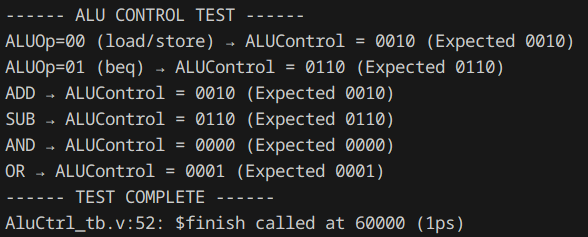
\includegraphics[width=0.6\linewidth]{aluctrl.png}
                    \caption{Sample Testbench output of ALU Control Unit}
                    \label{fig:placeholder}
                \end{figure}

            \subsection{The Arithmetic Logic Unit (ALU):-}
            \begin{itemize}
                \item Receives the 4-bit instruction from ALU control Unit.
                \item Executes operations on the data fetched from registers.
                \item Operations may include arithmetic (add, subtract), logical (AND, OR), or address calculation (base + offset).
                \begin{figure}[H]
                    \centering
                    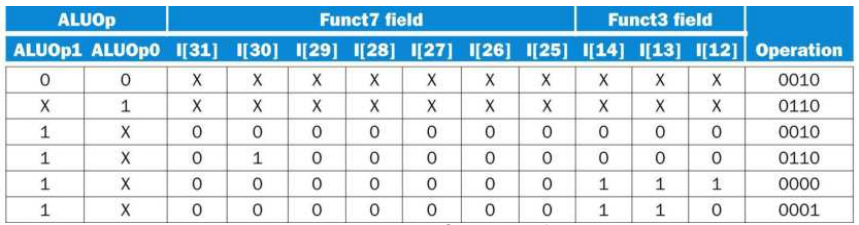
\includegraphics[width=0.8\linewidth]{att.png}
                    \caption{ALU truth table}
                    \label{fig:placeholder}
                \end{figure}
            \end{itemize}
            \subsubsection*{\textbf{Verification:-}}
            The module has been implemented in verilog and has been verified with an appropriate test bench. The output verifying the test-cases is as follows:-
                \begin{figure}[H]
                    \centering
                    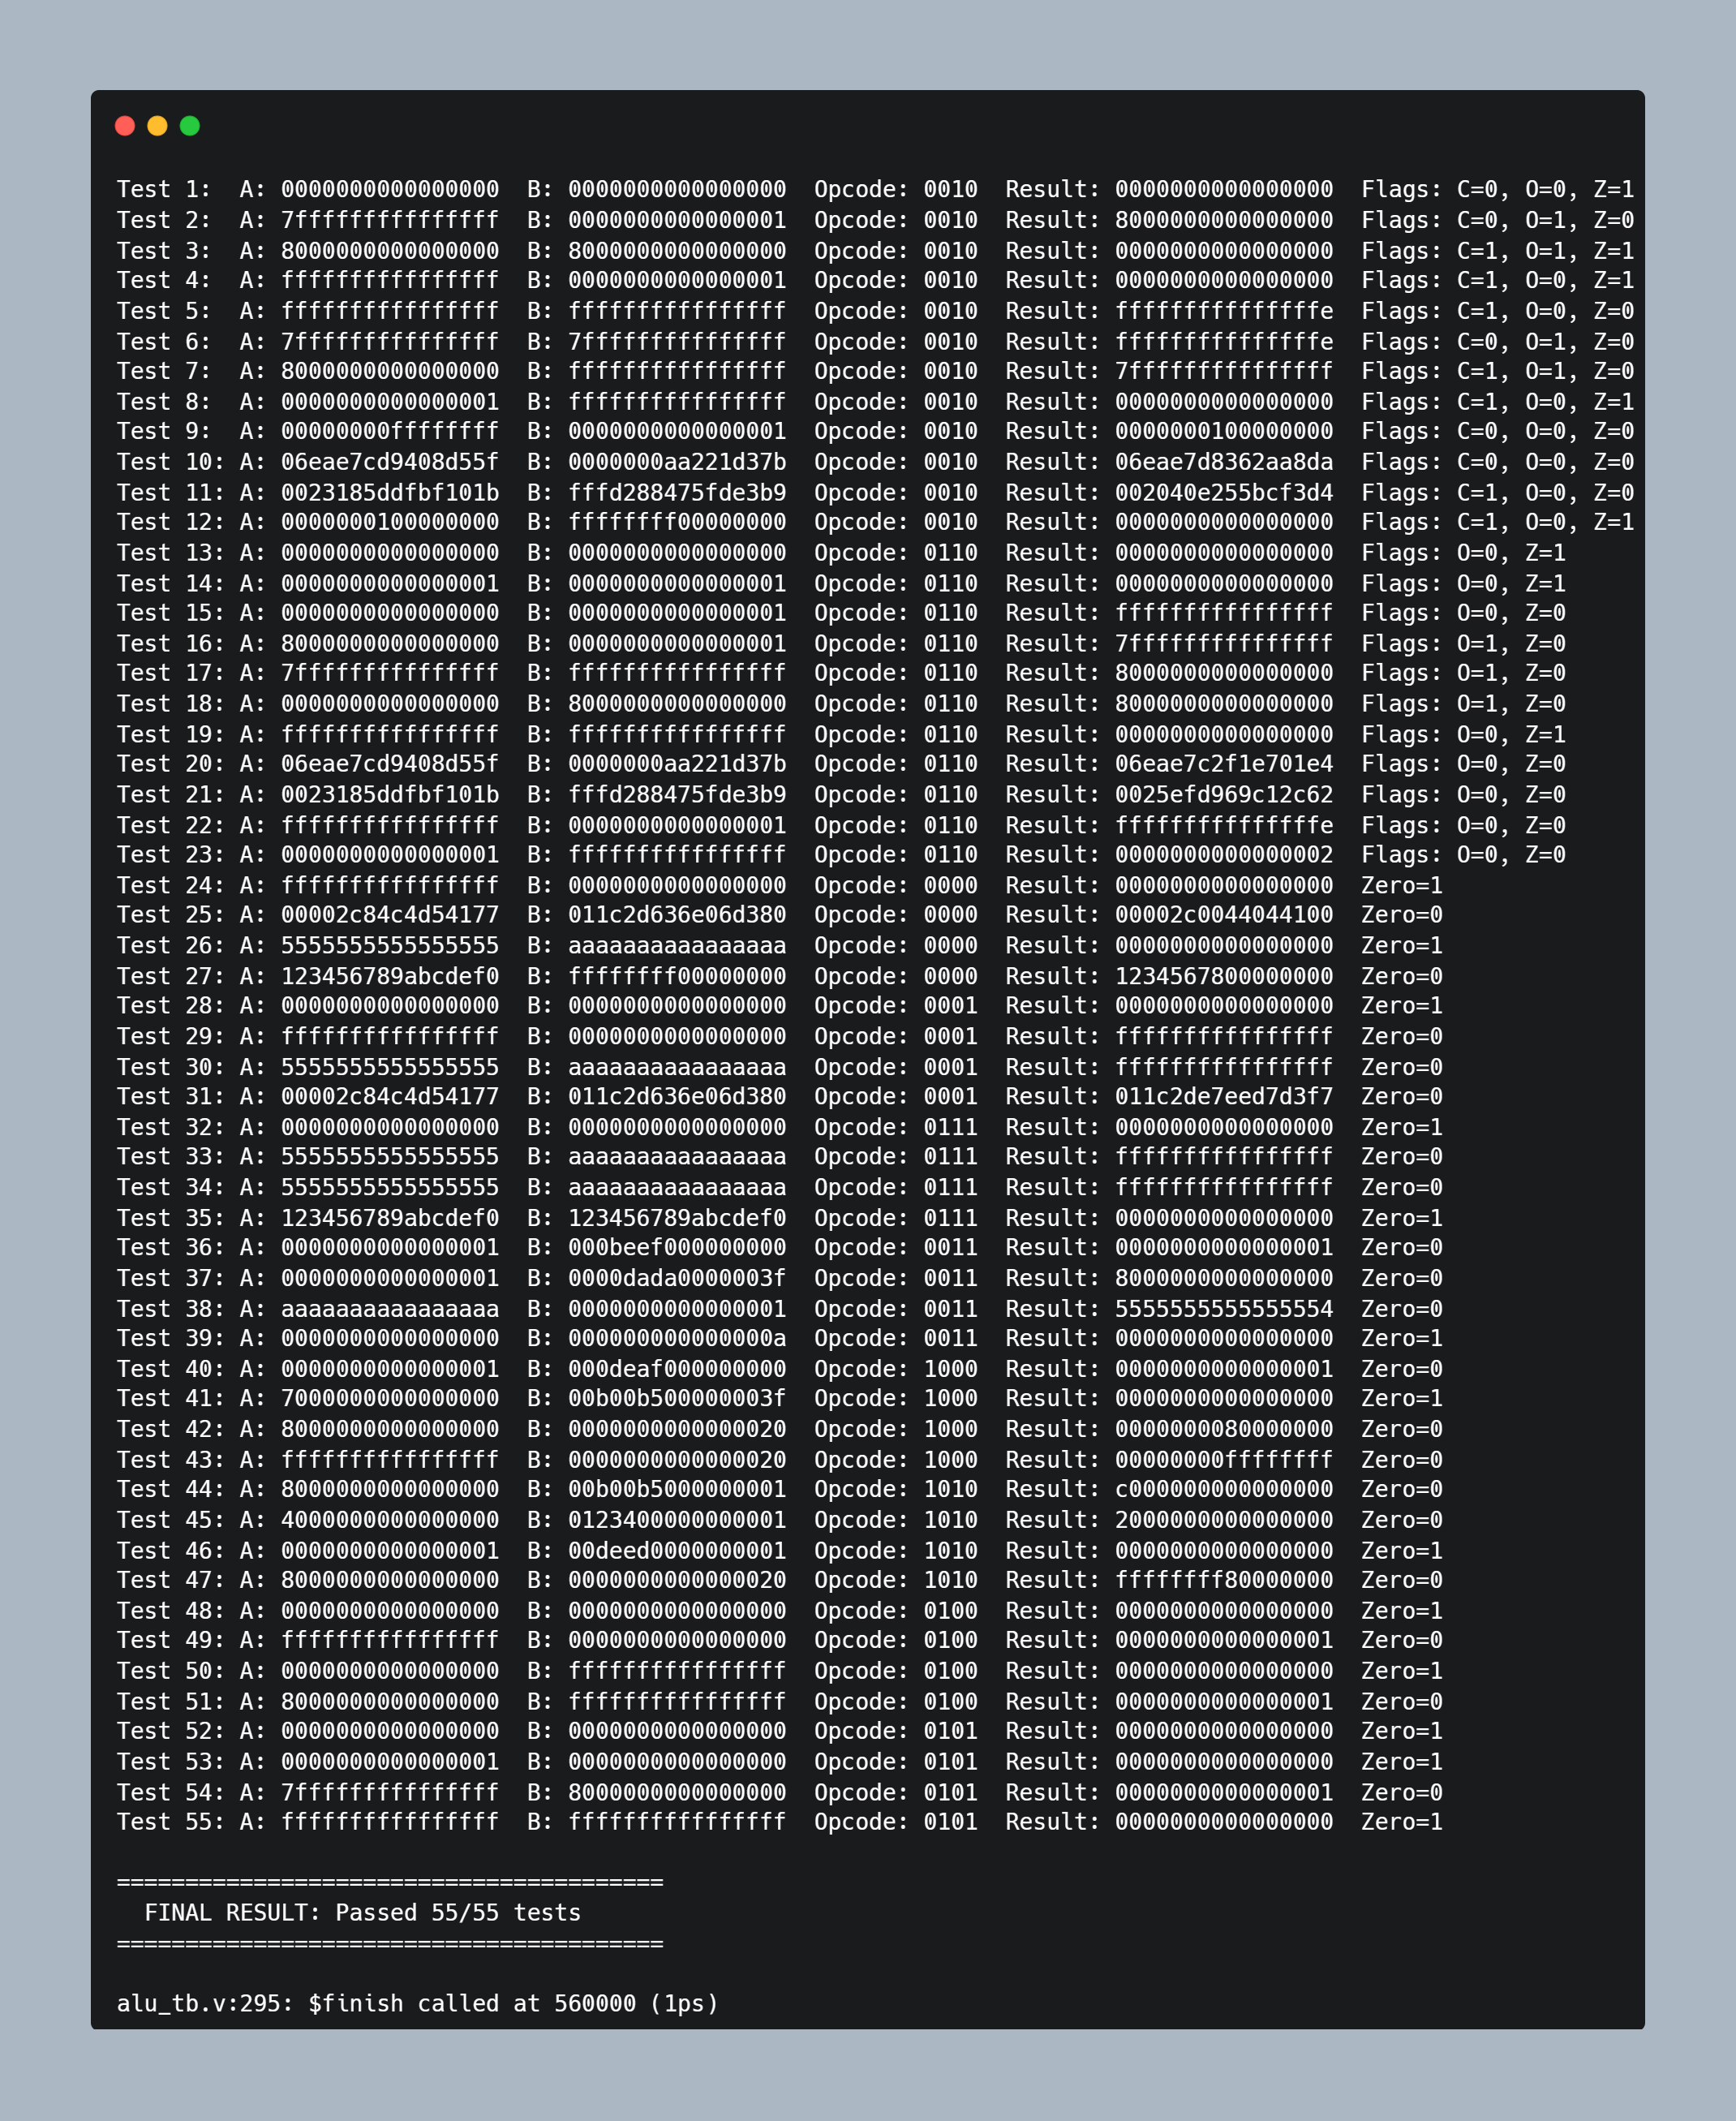
\includegraphics[width=0.6\linewidth]{ALU_test.png}
                    \caption{Sample Testbench output of ALU}
                    \label{fig:placeholder}
                \end{figure}
                \begin{figure}[H]
                    \centering
                    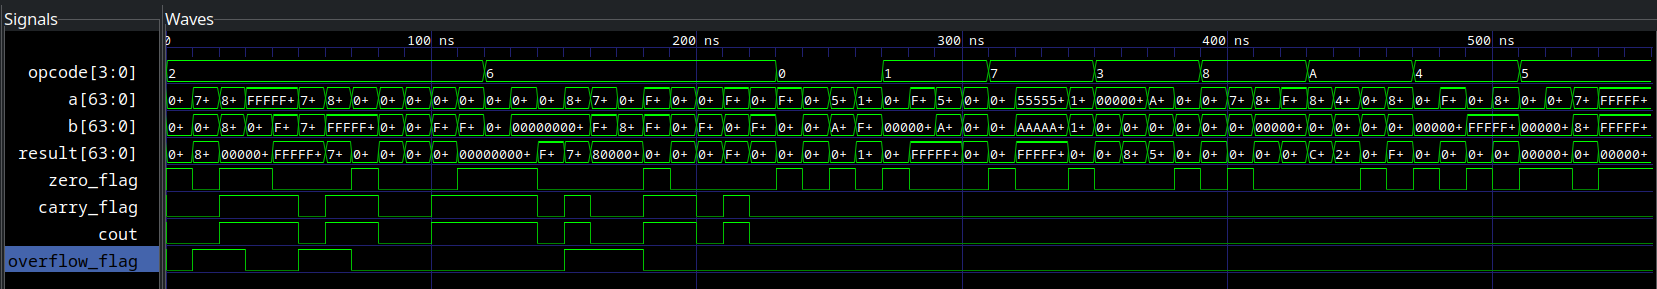
\includegraphics[width=0.6\linewidth]{alugtk.png}
                    \caption{GTKwave of ALU}
                    \label{fig:placeholder}
                \end{figure}
                
\section{Stage 4: Memory Access}

\begin{figure}[h]
    \centering
    \fbox{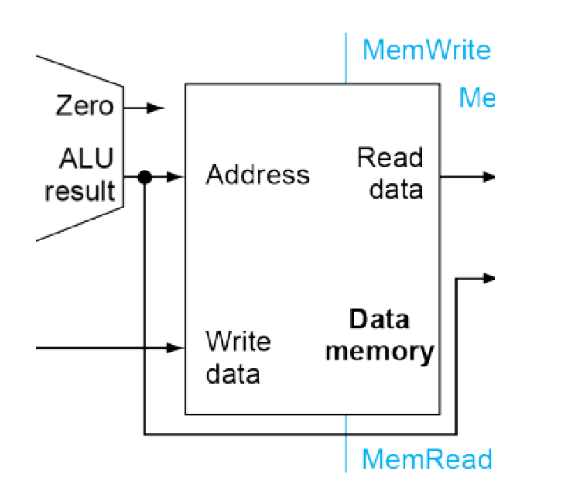
\includegraphics[width=0.5\linewidth]{Stage 4.png}}
    \caption{Memory access}
    \label{fig:placeholder}
\end{figure}
\subsection{Memory Access Behavior}
    \subsubsection*{Load Instructions (LD)}
        \begin{itemize}
            \item The effective memory address is computed as the \textit{ALU result}.
            \item The processor reads 64 bits from Data Memory at the computed address.
            \item The data becomes available at the beginning of the next clock cycle.
            \item This value is written back into the destination register during the Write-Back stage.
        \end{itemize}

    \subsubsection*{Store Instructions (SD)}
        \begin{itemize}
            \item The effective memory address is computed as the \textit{ALU result}.
            \item The processor writes 64 bits from a source register into Data Memory at this address.
            \item No value is written back into the register file.
            \item The next instruction proceeds without any additional write-back activity.
        \end{itemize}
    \subsubsection*{All Other Instructions}
    \begin{itemize}
        \item The Memory Access stage performs no operation.
        \item The ALU output is forwarded directly to the Write-Back multiplexer.  
    \end{itemize}

\subsection{Role of \texttt{MemRead} and \texttt{MemWrite}}
    These control signals originate from the Control Unit based on the instruction's opcode:
    \begin{itemize}
        \item \texttt{MemRead} = 1: The instruction requires reading from Data Memory (e.g., \texttt{ld}).
        \item \texttt{MemWrite} = 1: The instruction requires writing to Data Memory (e.g., \texttt{sd}).
    \end{itemize}
\begin{figure}[H]
    \centering
    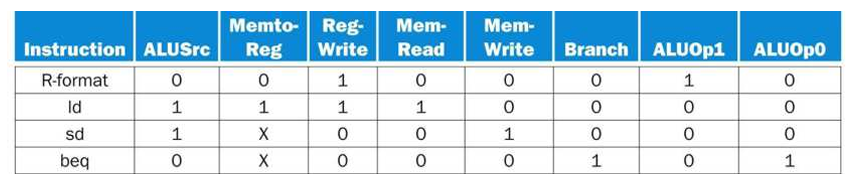
\includegraphics[width=1\linewidth]{Controls.png}
    \caption{opcodes of the Instructions}
    \label{fig:placeholder}
\end{figure}

\subsubsection*{\textbf{Verification:-}}
            The module has been implemented in verilog and has been verified with an appropriate test bench. The output verifying the test-cases is as follows:-
             \begin{figure}[H]
                    \centering
                    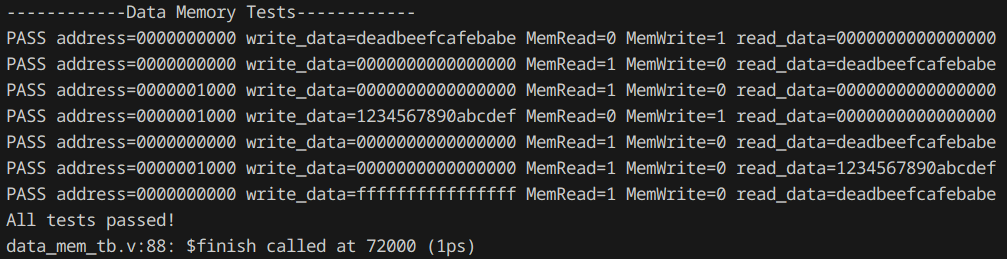
\includegraphics[width=0.6\linewidth]{datamem.png}
                    \caption{Sample Testbench output of Data Memory module}
                    \label{fig:placeholder}
                \end{figure}
                 \begin{figure}[H]
                    \centering
                    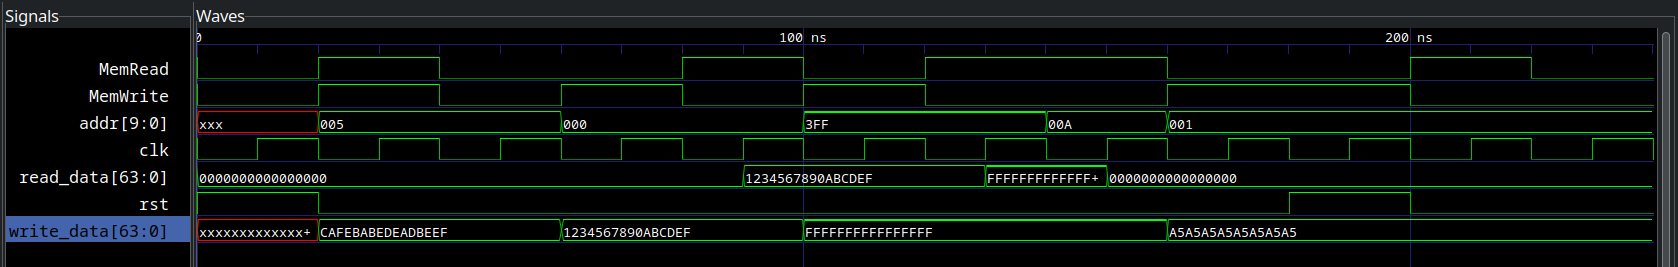
\includegraphics[width=0.7\linewidth]{datamemgtk.png}
                    \caption{GTKwave of Data Memory module}
                    \label{fig:placeholder}
                \end{figure}

\section{Stage 5: Write Back}
\begin{figure}[H]
    \centering
    \fbox{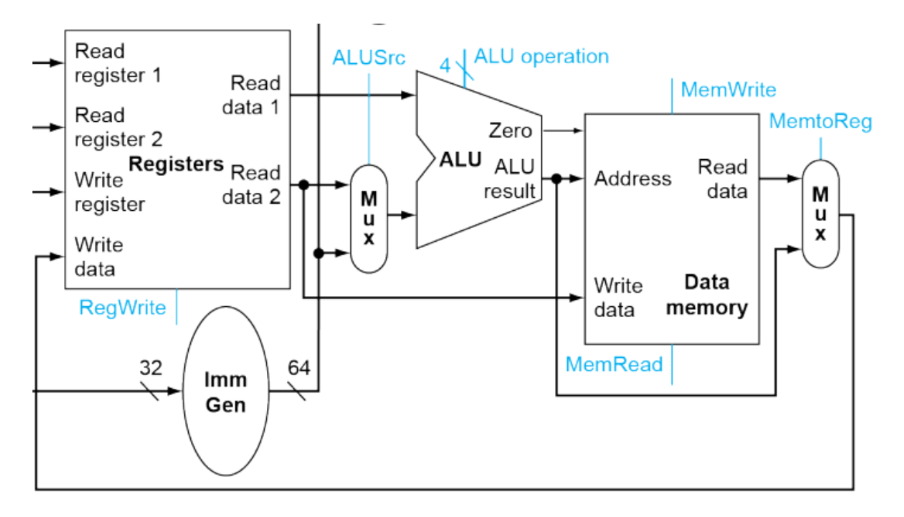
\includegraphics[width=0.7\linewidth]{Stage 5.png}}
    \caption{Write back into the register file}
    \label{fig:placeholder}
\end{figure}
    \begin{itemize}
    \item The final output of an instruction is written to the Register File.
    \begin{itemize}
        \item For ALU instructions, the value produced by the ALU is written to the destination register.
        \item For load instructions, the value retrieved from Data Memory is written back instead.
    \end{itemize}

    \item A multiplexer at the end of the datapath selects whether the Write-Back stage receives the ALU result or the memory output.

    \item The \texttt{RegWrite} signal generated by the Control Unit enables the register file to store the selected value.
\end{itemize}


\section{Implementation of Fibonacci Sequence Code}
We tested our code with a simple iterative version of the first ten elements of the Fibonacci series. The assembly code for implementing this is as shown below.

\begin{lstlisting}
    addi x1, x0, 10       /* Calculate 10 Fibonacci numbers*/
    addi x2, x0, 0        /* Address for storing results*/
    addi x3, x0, 0        /* Fib(0) = 0*/
    addi x4, x0, 1        /* Fib(1) = 1*/
    sd x3, 0(x2)          /* Store Fib(0)*/
    addi x2, x2, 8        /* Increment address (changed from 8)*/
    sd x4, 0(x2)          /* Store Fib(1)*/
    addi x2, x2, 8        /* Increment address (changed from 8)*/
    addi x5, x0, 2        /* i = 2*/
loop:
    beq x5, x1, done
    add x6, x3, x4
    sd x6, 0(x2)
    addi x2, x2, 8
    addi x5, x5, 1
    add x3, x0, x4
    add x4, x0, x6
    beq x0, x0, loop
done:
    add x2, x0, x0        /*iterating address for loading*/
    ld x10, 0(x2)         /*put the series onto the registers (x10-x19)*/
    ld x11, 8(x2)
    ld x12, 16(x2)
    ld x13, 24(x2)
    ld x14, 32(x2)
    ld x15, 40(x2)
    ld x16, 48(x2)
    ld x17, 56(x2)
    ld x18, 64(x2)
    ld x19, 72(x2)
\end{lstlisting}

At the end of the code we are expected to see registers 10-19 be filled with the first 10 values of the Fibonacci series, which is seen in the output file as follows:
\begin{lstlisting}
0000000000000000
000000000000000a
0000000000000000
0000000000000015
0000000000000022
000000000000000a
0000000000000022
0000000000000000
0000000000000000
0000000000000000
0000000000000000
0000000000000001
0000000000000001
0000000000000002
0000000000000003
0000000000000005
0000000000000008
000000000000000d
0000000000000015
0000000000000022
0000000000000000
0000000000000000
0000000000000000
0000000000000000
0000000000000000
0000000000000000
0000000000000000
0000000000000000
0000000000000000
0000000000000000
0000000000000000
0000000000000000
86
\end{lstlisting}
The waveform of different control signals, instruction and program counter are plotted to show an instant where the code takes a branch and executes the same set of instructions again is shown below:
\begin{figure}[H]
    \centering
        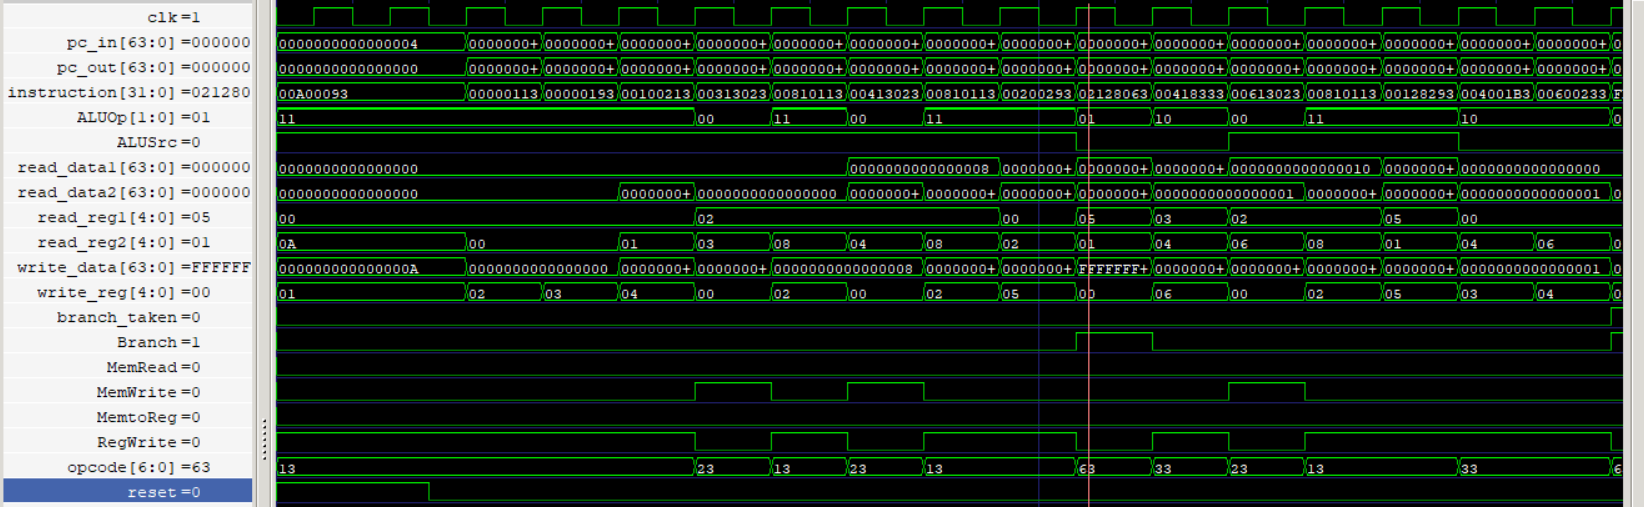
\includegraphics[width=1.2\linewidth]{fibonacci_out.png}
    \caption{Waveform showing an instant of execution of the fibonacci program.}
    \label{fig:fib-verify}
\end{figure}
\noindent This concludes our processor's design and verification of the same.\\
\noindent\makebox[\textwidth][l]{\rule{\dimexpr\textwidth+2cm}{1pt}}
\end{document}
